% !TEX root = Simulation.tex

\chapter{Fractals - Text Chapter 7}

\section{Problem 10}
\textbf{
Implement a bracketed OL-system and reproduce all plant-like structures of Figure~7.24 in the text. Change some derivation rules and see what happens. Make your own portfolio with at least ten plants.
}

\hfill \\

The first step to solving this problem was to gather the necessary test input. The parameters from Figure~7.24 in the text were summarized into Figure~\ref{7.24_rep}. The images were created using the program developed for the problem.

After collecting the necessary data, I saw two distinct parts to this problem. One was to create the L-system strings, and the other was to interpret them using Python's Turtle graphics (as suggested).

\subsection{L-system generation}
L-systems are rather straight forward so I made a simple class to encapsulate them. I tested this class against the example in section 7.4.3 in the text. The code can be found in Listing~\ref{LSystem.py} and the results can be found in Figure~\ref{lsystem_results}.

\begin{figure}
\centering
\includegraphics[scale=.75]{LSystemResults}
\caption{LSystem Results}
\label{lsystem_results}
\end{figure}


\subsection{Turtle Graphics representation}
Generating the actual Python turtle code was also simple. I encapsulated the process in a class called LSystemTurtle that would initialize, run, and save the results from each L-system. This code can be found in Listing~\ref{LSystemTurtle.py}. The default function run if this python file is run generated the six example images seen in Figure~\ref{7.24_rep}. It's worth noting that even with the turtle speed set to 0 (meaning no animation), these plants took a very long time to reproduce\footnote{Like, "I could have grown a real tree faster than this" very long time}.

After generating the given examples the task was to mess with the parameters to create a portfolio of ten different plants. Below I'll list my thought processes for each of the plants in the portfolio found in Appendix~\ref{plant_portfolio}. For the last two, I had to modify my code slightly. The modification amounted to checking if the d and delta variables were functions and if they were calling them instead of using them as normal. You can see this around lines 24, 40, and 45 in the code. The code to actually create the portfolio can be seen in Listing~\ref{PlantPortfolio.py}.

\subsubsection{Symmetrical G}
For this plant, I decided to keep the $F \rightarrow FF$ parameter and just adapt the $G$ parameter. I like symmetry so my thought was to make a string that is a palindrome and use that as the replacement in G. The full set of parameters I decided to go with was:

\begin{center}
$\begin{aligned}
& t = 4, \delta = 22.5\degree \\
& \omega = G \\
& G \rightarrow GG+[GF-][-FG]+GG
& F \rightarrow FF
\end{aligned}$
\end{center}

\subsubsection{Symmetrical G with +/- swapping}
For this plant, I kept the same parameters as the previous one, but instead of being a true palindrome, I swapped the + and - signs on the second half of the G parameter. This gave me:

\begin{center}
$\begin{aligned}
& t = 4, \delta = 22.5\degree \\
& \omega = G \\
& G \rightarrow GG+[GF-][+FG]-GG
& F \rightarrow FF
\end{aligned}$
\end{center}

\subsubsection{Symmetrical F only}
In this parameter set, I removed the G parameter and went with only one parameter to choose from. Again, I wanted to experiment with symmetry so I went with a palindrome.

\begin{center}
$\begin{aligned}
& t = 4, \delta = 22.5\degree \\
& \omega = 'F' \\
& F \rightarrow FF+[-F[--F][F--]F-]+FF
\end{aligned}$
\end{center}

\subsubsection{Symmetrical F only with +/- swapping}
This time I used the same single parameter set as the previous plant but swapped the + and - signs in the second half of the palindrome.

\begin{center}
$\begin{aligned}
& t = 4, \delta = 22.5\degree \\
& \omega = 'F' \\
& F \rightarrow FF+[-F[--F][F++]F+]-FF
\end{aligned}$
\end{center}

\subsubsection{Turning F}
For this plant I wanted to make a very asymmetrical plant. My plan for this was to have the F parameter constantly turn in one direction. This plant is directly modified from the plant in Figure~\ref{7.24_rep}(c).

\begin{center}
$\begin{aligned}
& t = 4, \delta = 22.5\degree \\
& \omega = G \\
& G \rightarrow F[+FFG][G]-FG \\
& F \rightarrow FF-FFF
\end{aligned}$
\end{center}

\subsubsection{Symmetrical Turning F}
This time I wanted to try having a palindrome with turns for the F value. This one is again adapted from Figure~\ref{7.24_rep}(c).

\begin{center}
$\begin{aligned}
& t = 4, \delta = 22.5\degree \\
& \omega = G \\
& G \rightarrow F[+FFG][G]-FG \\
& F \rightarrow FF-F-FF
\end{aligned}$
\end{center}

\subsubsection{Symmetrical Turning F with +/- swapping}
This one is adapted from the above plant with the second - sign being replaced with a +. The hope was that this would produce a "wavy" plant.

\begin{center}
$\begin{aligned}
& t = 4, \delta = 22.5\degree \\
& \omega = G \\
& G \rightarrow F[+FFG][G]-FG \\
& F \rightarrow FF-F+FF
\end{aligned}$
\end{center}

\subsubsection{Similar G \& F}
For this plant, I wanted to see what happens when F and G are similar, but with the Fs and Gs in them swapped.

\begin{center}
$\begin{aligned}
& t = 4, \delta = 22.5\degree \\
& \omega = G \\
& G \rightarrow FF-G[+GF]G \\
& F \rightarrow GG-F[+FG]F
\end{aligned}$
\end{center}

\subsubsection{Randomized distance}
In an attempt to get a random plant, I decided to make the distance stepped at each point be determined randomly. The other parameters where taken from Figure~\ref{7.24_rep}(b).

\begin{center}
$\begin{aligned}
& t = 4, \delta = 22.5\degree \\
& \omega = F \\
& F \rightarrow FF+[+F-F-F]-[-F+F+F]
\end{aligned}$
\end{center}

\subsubsection{Randomized turn ($\delta$)}
In another attempt to get a random plant, I decided to make the angle turned at each point be determined randomly. The other parameters where taken from Figure~\ref{7.24_rep}(b).

\begin{center}
$\begin{aligned}
& t = 4, \delta_i = random_i(20.0, 30.0) \\
& \omega = F \\
& F \rightarrow FF+[+F-F-F]-[-F+F+F]
\end{aligned}$
\end{center}

\begin{figure}
\centering
\begingroup \everymath{\scriptsize} \setlength{\medmuskip}{0mu}
\begin{tabular}{ | c | c | c | }
\hline
%\includegraphics[width=.3\linewidth]{LSystemExamples/lsystem_a} &
%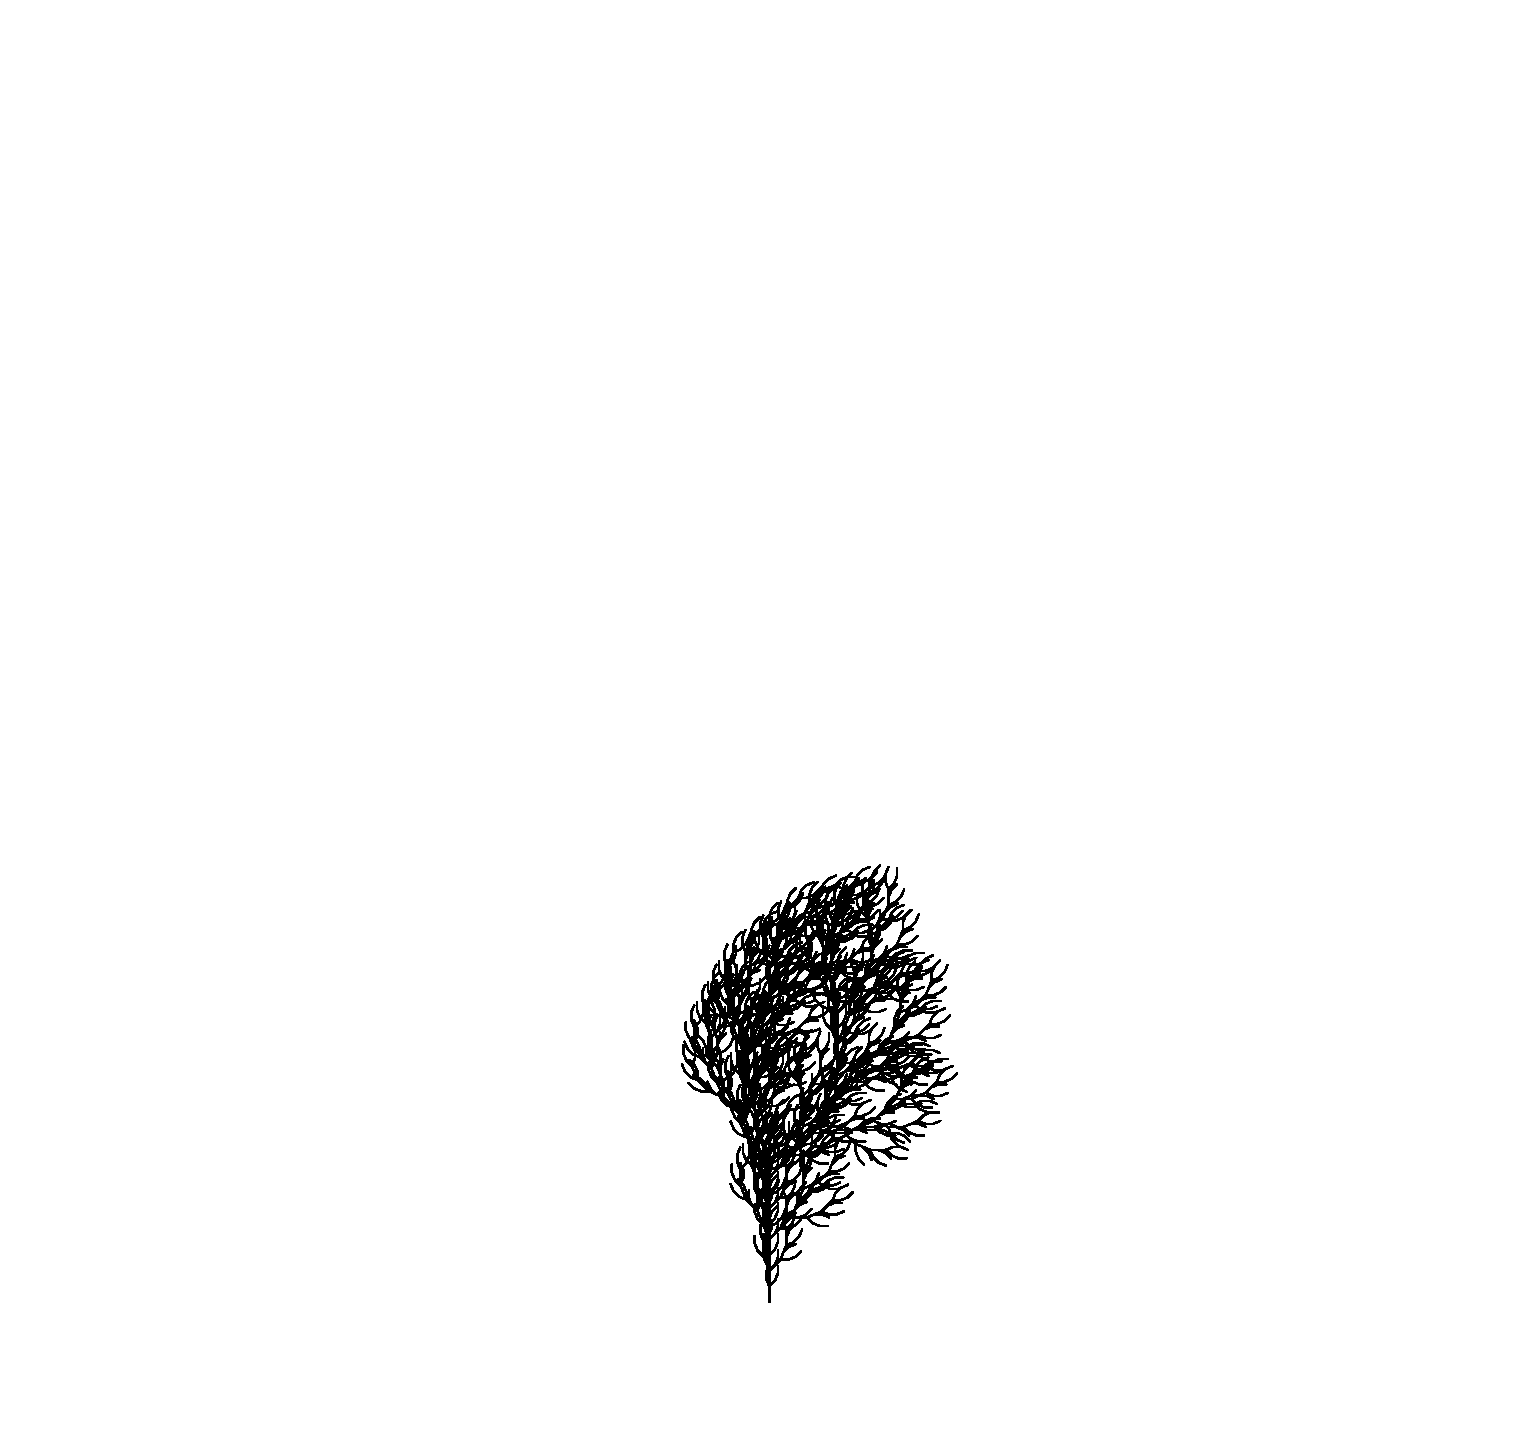
\includegraphics[width=.3\linewidth]{LSystemExamples/lsystem_b} &
%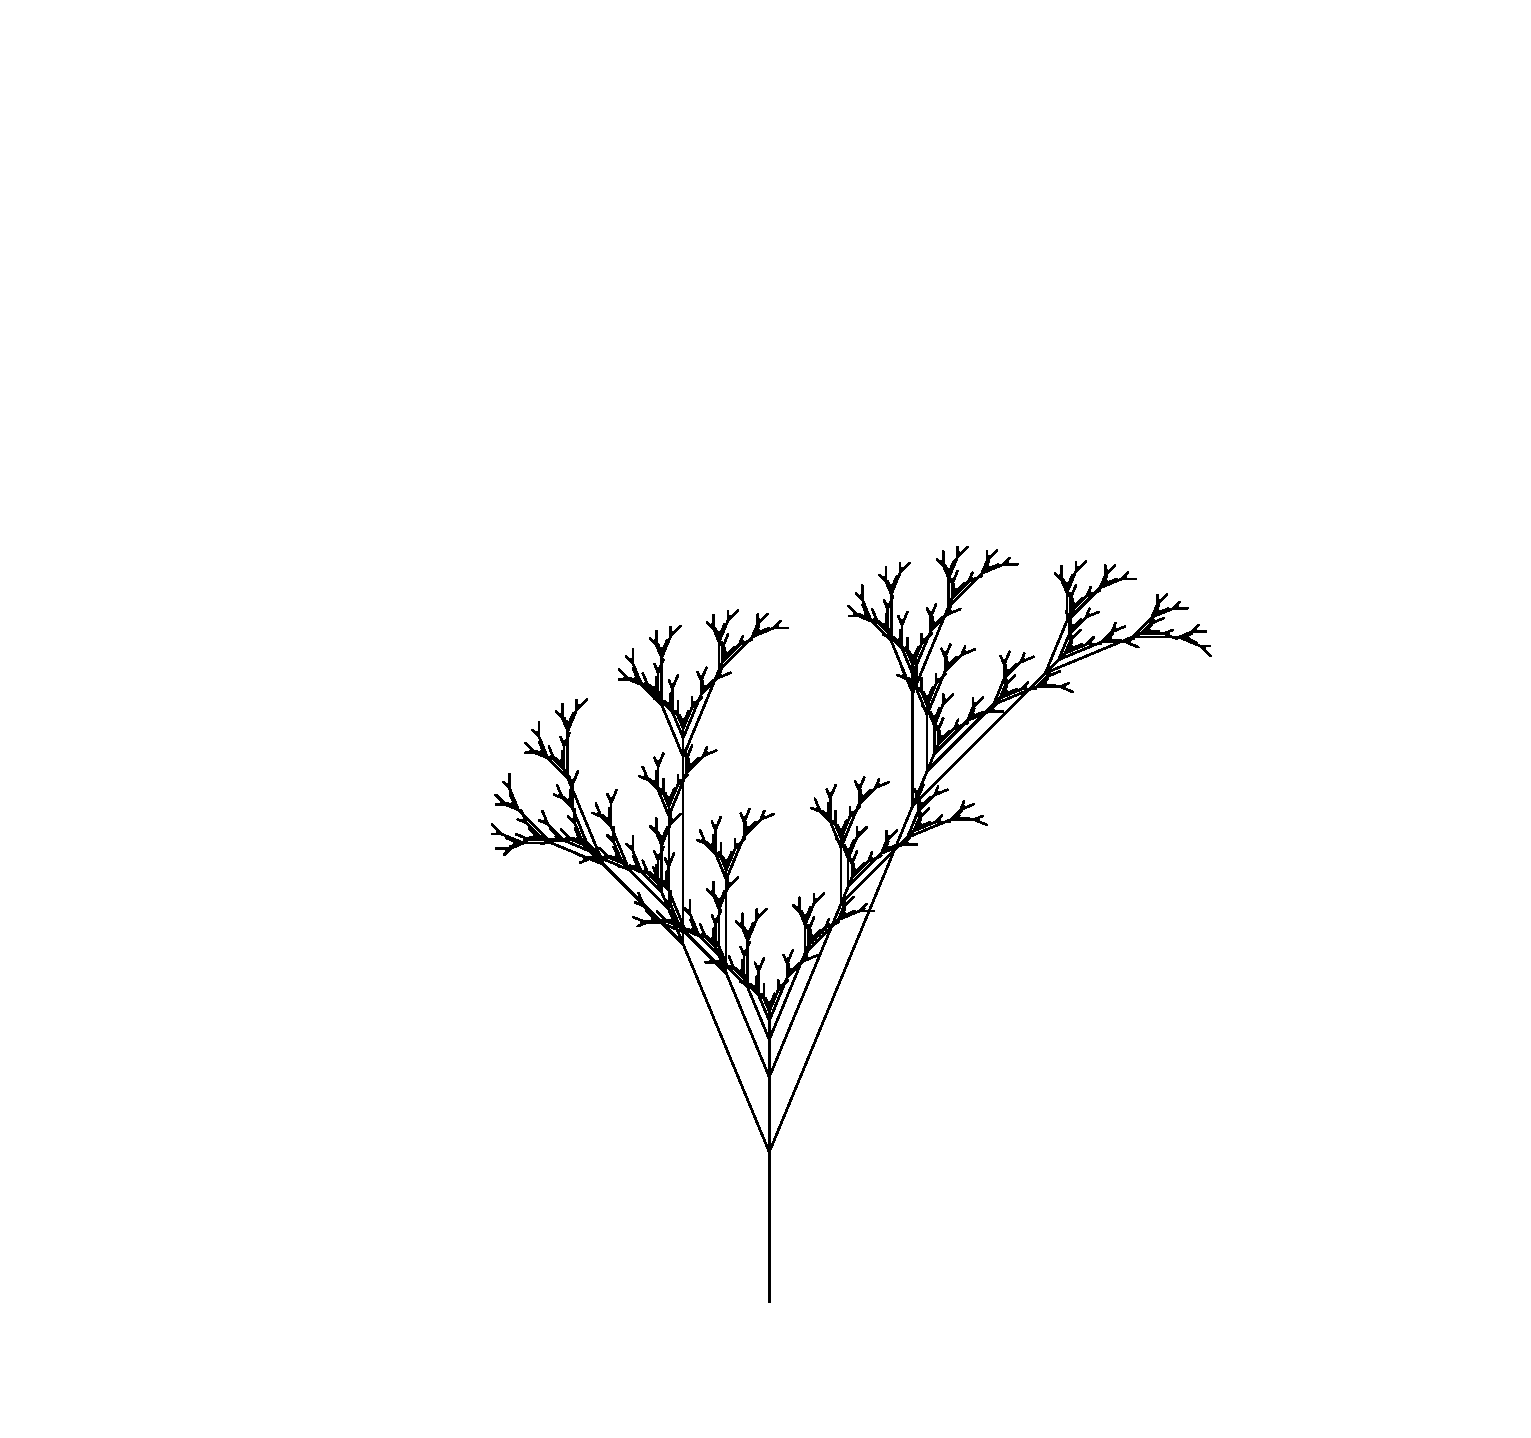
\includegraphics[width=.3\linewidth]{LSystemExamples/lsystem_c} \\

$\begin{aligned}
& t = 8, \delta = 22.5\degree \\
& \omega = G \\
& G \rightarrow F+[[G]-G]-F[-FG]+G \\
& F \rightarrow FF
\end{aligned}$ & 
$\begin{aligned}
& t = 4, \delta = 22.5\degree \\
& \omega = F \\
& F \rightarrow FF+[+F-F-F]-[-F+F+F]
\end{aligned}$ & 
$\begin{aligned}
& t = 6, \delta = 22.5\degree \\
& \omega = G \\
& G \rightarrow F[+FFG][G]-FG \\
& F \rightarrow FF
\end{aligned}$ \\ \hline

%\includegraphics[width=.3\linewidth]{LSystemExamples/lsystem_d} &
%\includegraphics[width=.3\linewidth]{LSystemExamples/lsystem_e} &
%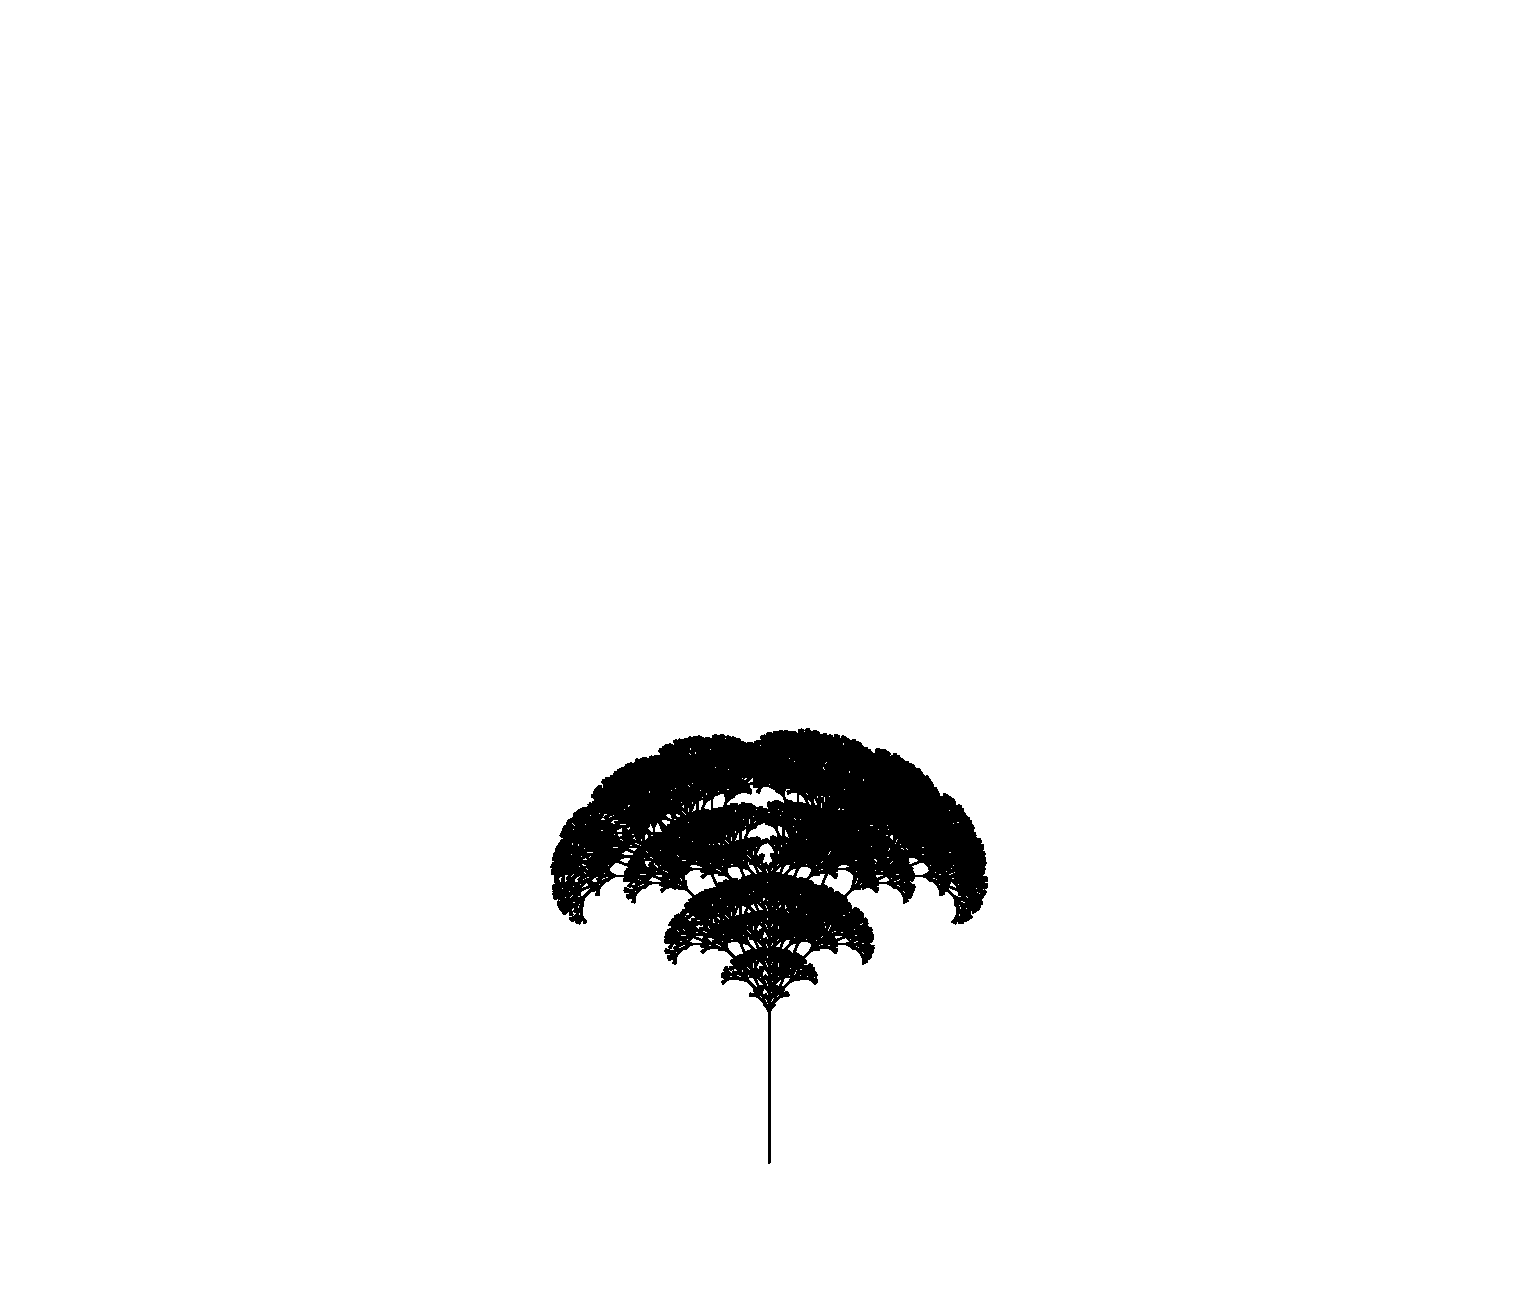
\includegraphics[width=.3\linewidth]{LSystemExamples/lsystem_f} \\

$\begin{aligned}
& t = 9, \delta = 20\degree \\
& \omega = G \\
& G \rightarrow F[-G]F[+G]-G \\
& F \rightarrow FF
\end{aligned}$ &
$\begin{aligned}
& t = 9, \delta = 25.7\degree \\
& \omega = G \\
& G \rightarrow F[-G][+G]FG \\
& F \rightarrow FF
\end{aligned}$ &
$\begin{aligned}
& t = 5, \delta = 22.5\degree \\
& \omega = G \\
& G \rightarrow FG[-F[G]-G][G+G][+F[G]+G] \\
& F \rightarrow FF
\end{aligned}$ \\ \hline
\end{tabular}
\endgroup
\caption{Reproduction of figure 7.24 in the text}
\label{7.24_rep}
\end{figure}

\section{Problem 15}
\textbf{
Implement a random iterated function system (RIFS) to generate all the fractals whose codes are presented in Table~7.3 in the text.
}

\hfill \\

Again, the first step was to reproduce the data needed for the problem. Table~7.3 from the text has been reproduced in Table~\ref{7.3_rep}.

With this data available I created a simple class to do the iterated functions, which would output a list of x and y values that I would plot after the full set was created. This is a slight (less graphics intensive) modification of Algorithm~7.3 in the text. This code can be seen in Listing~\ref{RIFS.py}. The resulting fractals can be seen in Appendix~\ref{RIFS_results}.

\begin{table}
\begin{tabular}{ c c }
	\begin{tabular}{ c c c c c c c c }
	\hline
	w & a & b & c & d\footnote{Corrected as suggested on assignment page} & e & f & p \\
	\hline
	1 & 0.5 & 0 & 0 & 0.5 & 1 & 1 & 0.33 \\
	2 & 0.5 & 0 & 0 & 0.5 & 1 & 50 & 0.33 \\
	3 & 0.5 & 0 & 0 & 0.5 & 50 & 50 & 0.34 \\
	\hline
	\multicolumn{8}{c}{Sierpinski Gasket}
	\end{tabular} &

	\begin{tabular}{ c c c c c c c c }
	\hline
	w & a & b & c & d & e & f & p \\
	\hline
	1 & 0.5 & 0 & 0 & 0.5 & 1 & 1 & 0.25 \\
	2 & 0.5 & 0 & 0 & 0.5 & 50 & 1 & 0.25 \\
	3 & 0.5 & 0 & 0 & 0.5 & 1 & 50 & 0.25 \\
	4 & 0.5 & 0 & 0 & 0.5 & 50 & 50 & 0.25 \\
	\hline
	\multicolumn{8}{c}{Square}
	\end{tabular} \\
	
	\hfill & \hfill \\
	
	\begin{tabular}{ c c c c c c c c }
	\hline
	w & a & b & c & d & e & f & p \\
	\hline
	1 & 0 & 0 & 0 & 0.16 & 0 & 0 & 0.01 \\
	2 & 0.85 & 0.04 & -0.04 & 0.85 & 0 & 1.6 &0.85 \\
	3 & 0.2 & -0.26 & 0.23 & 0.22 & 0 & 1.6 & 0.07 \\
	4 & -0.15 & 0.28 & 0.26 & 0.24 & 0 & 0.44 & 0.07 \\
	\hline
	\multicolumn{8}{c}{Barnsley Fern}
	\end{tabular} &
	
	\begin{tabular}{ c c c c c c c c }
	\hline
	w & a & b & c & d & e & f & p \\
	\hline
	1 & 0 & 0 & 0 & 0.5 & 0 & 0 & 0.05 \\
	2 & 0.42 & -0.42 & 0.42 & 0.42 & 0 & 0.2 & 0.40 \\
	3 & 0.42 & 0.42 & -0.42 & 0.42 & 0 & 0.2 & 0.40 \\
	4 & 0.1 & 0 & 0 & 0.1 & 0 & 0.2 & 0.15 \\
	\hline
	\multicolumn{8}{c}{Tree}
	\end{tabular}
\end{tabular}
\caption{Reproduction of Table 7.3 from the text}
\label{7.3_rep}
\end{table}

\section{Problem 21}
\textbf{
Implement the random midpoint displacement algorithm in 3D and generate some fractal landscapes. Study the influence of H on the landscapes generated.
}

\hfill \\
